\section{Résultats}
\label{sec:results}
Cette section présente les résultats de notre analyse empirique visant à évaluer l'impact de l'introduction de la taxe CO2 en Suisse en 2008 sur les émissions de gaz à effet de serre. Nous avons utilisé deux approches complémentaires pour garantir la robustesse de nos conclusions : la méthode de différence en différences (DiD) et la méthode de contrôle synthétique (SCM). Les résultats obtenus à partir de ces deux méthodes sont discutés en détail dans les sous-sections suivantes.

\subsection{Difference-In-Differences (DiD)}
\label{subsec:results_did}

Nous avons effectué une analyse de différence en différences (DiD) pour estimer l'impact causal de l'introduction de la taxe CO2 en Suisse en 2008 sur les émissions de CO2 par habitant. L'analyse a été réalisée à l'aide du logiciel Stata. Les résultats montrent un effet significatif de la taxe CO2 sur les émissions. En complément, nous avons également effectué un test des tendances parallèles pour vérifier la validité de notre approche. Ce test a révélé une divergence significative, indiquant une violation de l'hypothèse des tendances parallèles dans notre analyse.


\subsubsection{Résultats}
\label{subsubsec:results_did_table}



\begin{table}[H]
\centering
\tiny{
\begin{tabular}{lcc} \hline
 & (1) & (2) \\
VARIABLES & ATET & Controls \\ \hline
 &  &  \\
1995.year &  & -0.457 \\
 &  & (0.615) \\
1996.year &  & -0.293 \\
 &  & (0.121) \\
1997.year &  & -0.537 \\
 &  & (0.552) \\
1998.year &  & -0.207 \\
 &  & (0.548) \\
1999.year &  & -0.391 \\
 &  & (0.809) \\
2000.year &  & 0.458 \\
 &  & (0.917) \\
2001.year &  & -0.597 \\
 &  & (1.465) \\
2002.year &  & 0.242 \\
 &  & (0.514) \\
2003.year &  & 0.471 \\
 &  & (0.706) \\
2005.year &  & 0.290 \\
 &  & (0.406) \\
2006.year &  & 0.705 \\
 &  & (0.954) \\
2007.year &  & 0.637 \\
 &  & (1.114) \\
2008.year &  & 0.782 \\
 &  & (0.425) \\
2009.year &  & 0.423 \\
 &  & (0.336) \\
2010.year &  & 0.0743 \\
 &  & (1.107) \\
2011.year &  & 0.0112 \\
 &  & (0.667) \\
2012.year &  & 0.355* \\
 &  & (0.0290) \\
2013.year &  & 0.391 \\
 &  & (0.165) \\
2014.year &  & -0.114 \\
 &  & (0.370) \\
2015.year &  & -0.139 \\
 &  & (0.103) \\
2016.year &  & -0.177 \\
 &  & (0.0880) \\
2017.year &  & 0.0754 \\
 &  & (0.649) \\
2018.year &  & 0.257 \\
 &  & (1.129) \\
r1vs0.interaction & -1.263*** &  \\
 & (1.21e-08) &  \\
Constant &  & 7.795*** \\
 &  & (0.103) \\
 &  &  \\
 Observations & 48 & 48 \\ \hline
\multicolumn{3}{c}{ Robust standard errors in parentheses} \\
\multicolumn{3}{c}{ *** p$<$0.01, ** p$<$0.05, * p$<$0.1} \\
\end{tabular}
}
\caption{}
\label{tab:did_results_table}
\end{table}



% \footnotesize
Les résultats montrent un effet significatif de la taxe CO2 sur les émissions, comme le coefficient de l'interaction entre la variable indiquant la période post-intervention et la variable indiquant l'introduction de la taxe est négatif et statistiquement significatif (-1.263 tonnes CO$_2$ par habitant). Cela suggère que la taxe a eu un effet réducteur sur les émissions de CO2 en Suisse. Cependant, pour établir une relation causale robuste, il est essentiel de vérifier l'hypothèse des tendances parallèles (PT).


\subsubsection{Test sur les \hyperref[subsec:linear_trend_method]{tendances parallèles}}

\label{subsubsec:pt_test}

Pour évaluer la validité de notre analyse de différence en différences (DiD), nous avons effectué un test des \hyperref[subsec:linear_trend_method]{tendances parallèles}. Les graphiques sur la figure \ref{fig:omeans} et la figure \ref{fig:pt_test} ci-après présentent visuellement les tendances des émissions de CO2 par habitant pour la Suisse et l'Autriche avant l'introduction de la taxe CO2 en 2008. Ces graphiques des moyennes observées et des tendances linéaires sont complémentaires pour l'analyse et fournissent une évaluation visuelle cruciale de l'hypothèse des tendances parallèles.


\begin{figure}[H]
\centering
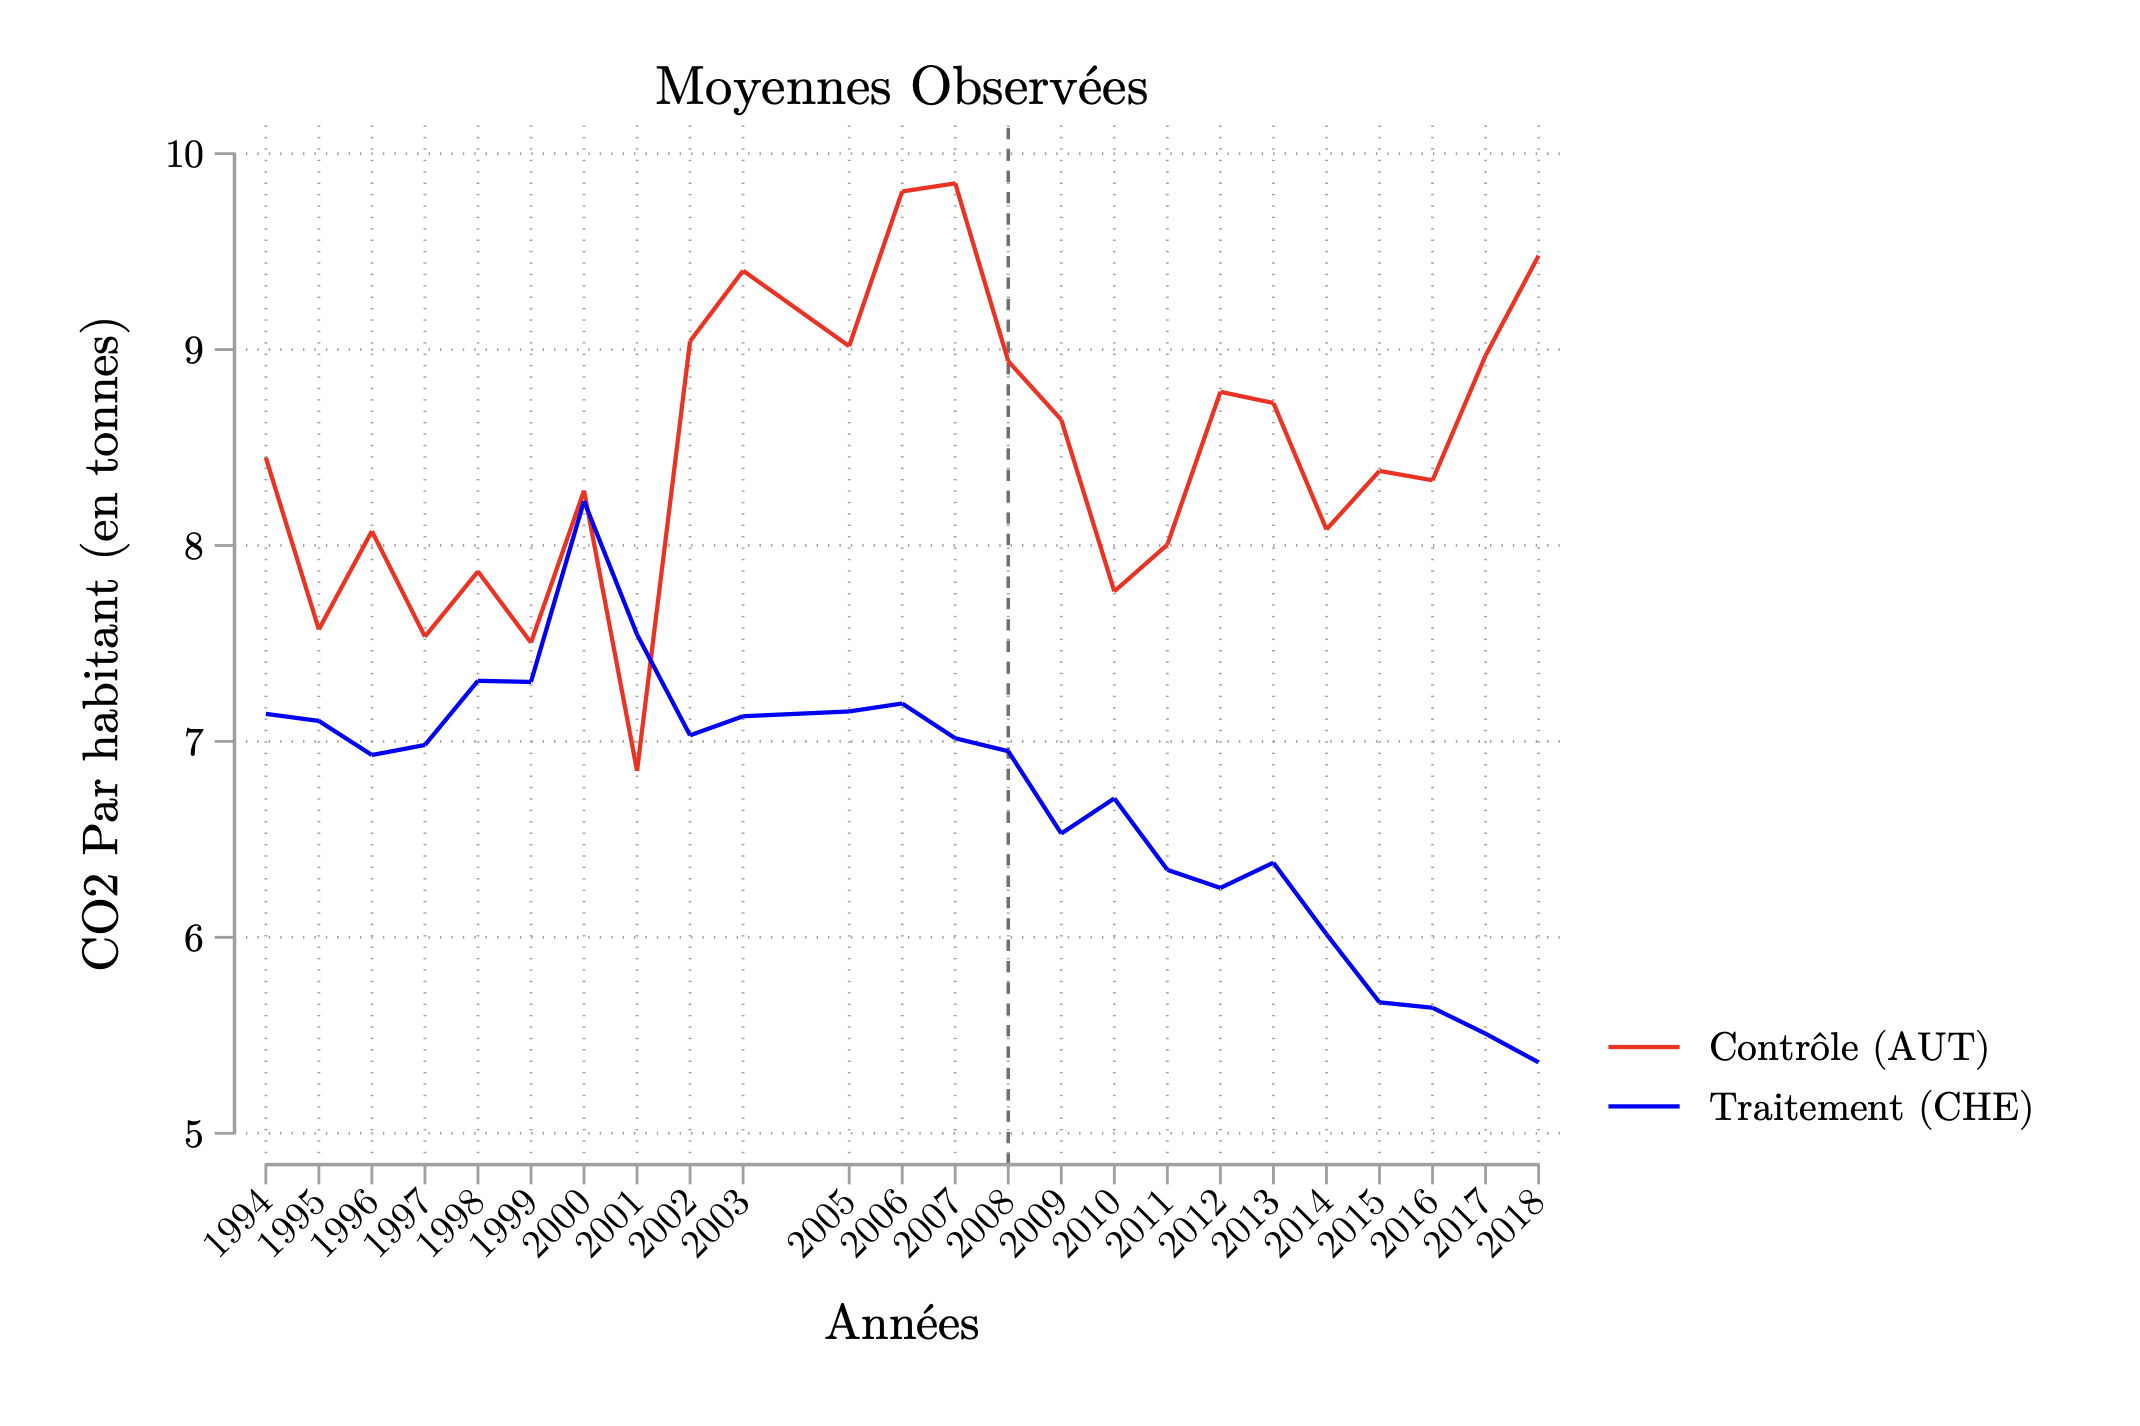
\includegraphics[width=0.6\textwidth]{Article/images/pt_test_omeans.png}
\caption{}
\label{fig:omeans}
    \end{figure}

\vspace*{0.5cm}

\begin{figure}[H]
\centering
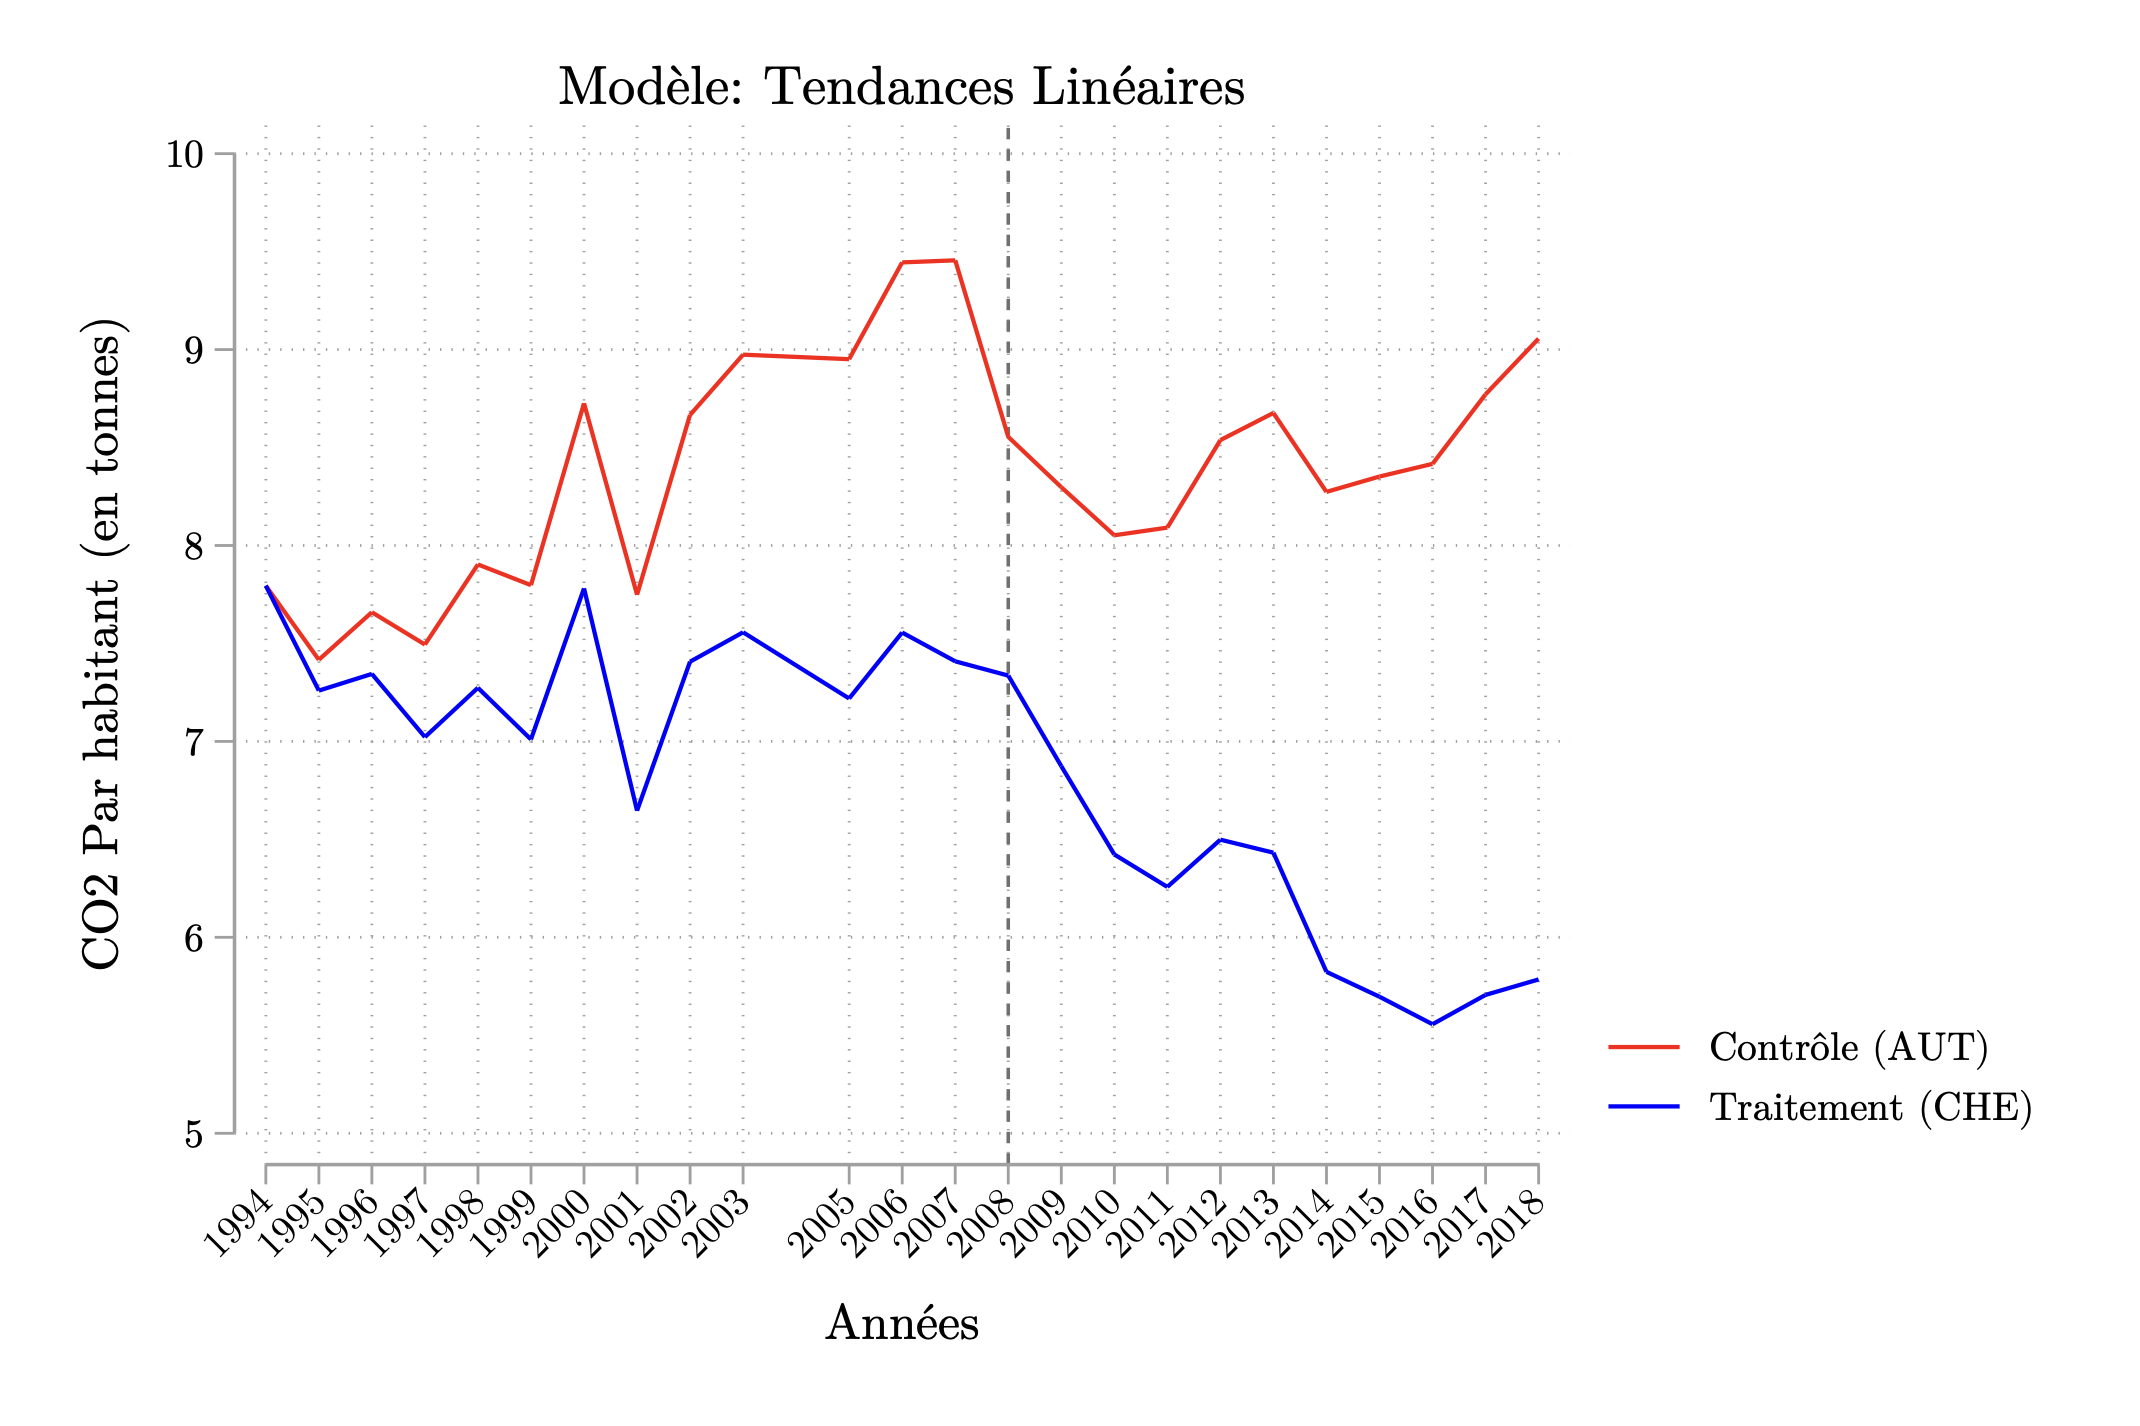
\includegraphics[width=0.6\textwidth]{Article/images/linear_trend_test.png}
\caption{}
\label{fig:pt_test}
    \end{figure}

    
En plus du graphique, nous présentons le  tableau$^{\left[\ref{tab:parallel_trends_test_table}\right]}$ ci-après contenant les résultats du test statistique des tendances parallèles. Les résultats montrent que les tendances des émissions de CO2 en Suisse et en Autriche ne sont pas parfaitement parallèles pendant la période pré-traitement. Cette absence de parallélisme est mise en évidence par un rejet significatif de l'hypothèse nulle, comme le montre une p-value de 0.000034506402586, indiquant une violation significative de l'hypothèse des tendances parallèles$^{\left[\ref{subsubsec:strategie_did_hypothesis}\right]}$.


\begin{table}[H]
\centering
\footnotesize{
\begin{tabular}{|c|c|c|c|c|} 
\hline
N & F-statistic & df(m) & df(r) & p-value \\ \hline
48 & 340377524.3623716 & . & 1 & .000034506402586 \\ \hline
\end{tabular}
}
\caption{Résultats du test des tendances parallèles}
\label{tab:parallel_trends_test_table}
\end{table}

Ces résultats suggèrent que l'analyse DiD ne peut pas fournir une conclusion causale robuste sans vérifier l'hypothèse des tendances parallèles. Par conséquent, des méthodes complémentaires, comme la méthode de contrôle synthétique (SCM), sont nécessaires pour fournir une évaluation plus fiable de l'impact de la taxe CO2 en Suisse.


\subsection{Résultats de la méthode de contrôle synthétique (SCM)}
\label{subsec:results_scm}

Dans cette section, nous présentons les résultats de notre analyse utilisant la méthode de contrôle synthétique (SCM) \subsectionref{strategie_scm_method} . Cette méthode permet de créer un groupe de contrôle synthétique qui correspond aux caractéristiques de la Suisse avant l'introduction de la taxe CO2 en 2008. Pour notre analyse, nous avons sélectionné le Luxembourg et la Hollande comme pays de contrôle pour constituer ce groupe synthétique en raison de leurs similitudes avec la Suisse sur des variables clés.

\subsubsection{Résultats}
\label{subsec:results_scm_graph_table}

Nous présentons sur le graphique de la figure \ref{fig:scm_omeans} les moyennes observées qui inclut le pays contrefactuel constitué des pondérations de l'Autriche, du Luxembourg et de la Hollande, ainsi que les résultats de ces pondérations. En effet, le graphique de la figure \ref{fig:scm_omeans} des moyennes observées est très similaire au graphique de la figure \ref{fig:omeans} observé lors de la DID avec seulement l'Autriche comme pays de contrôle, compte tenu de la faible contribution de la Hollande et de la contribution nulle du Luxembourg.


\begin{figure}[H]
\centering
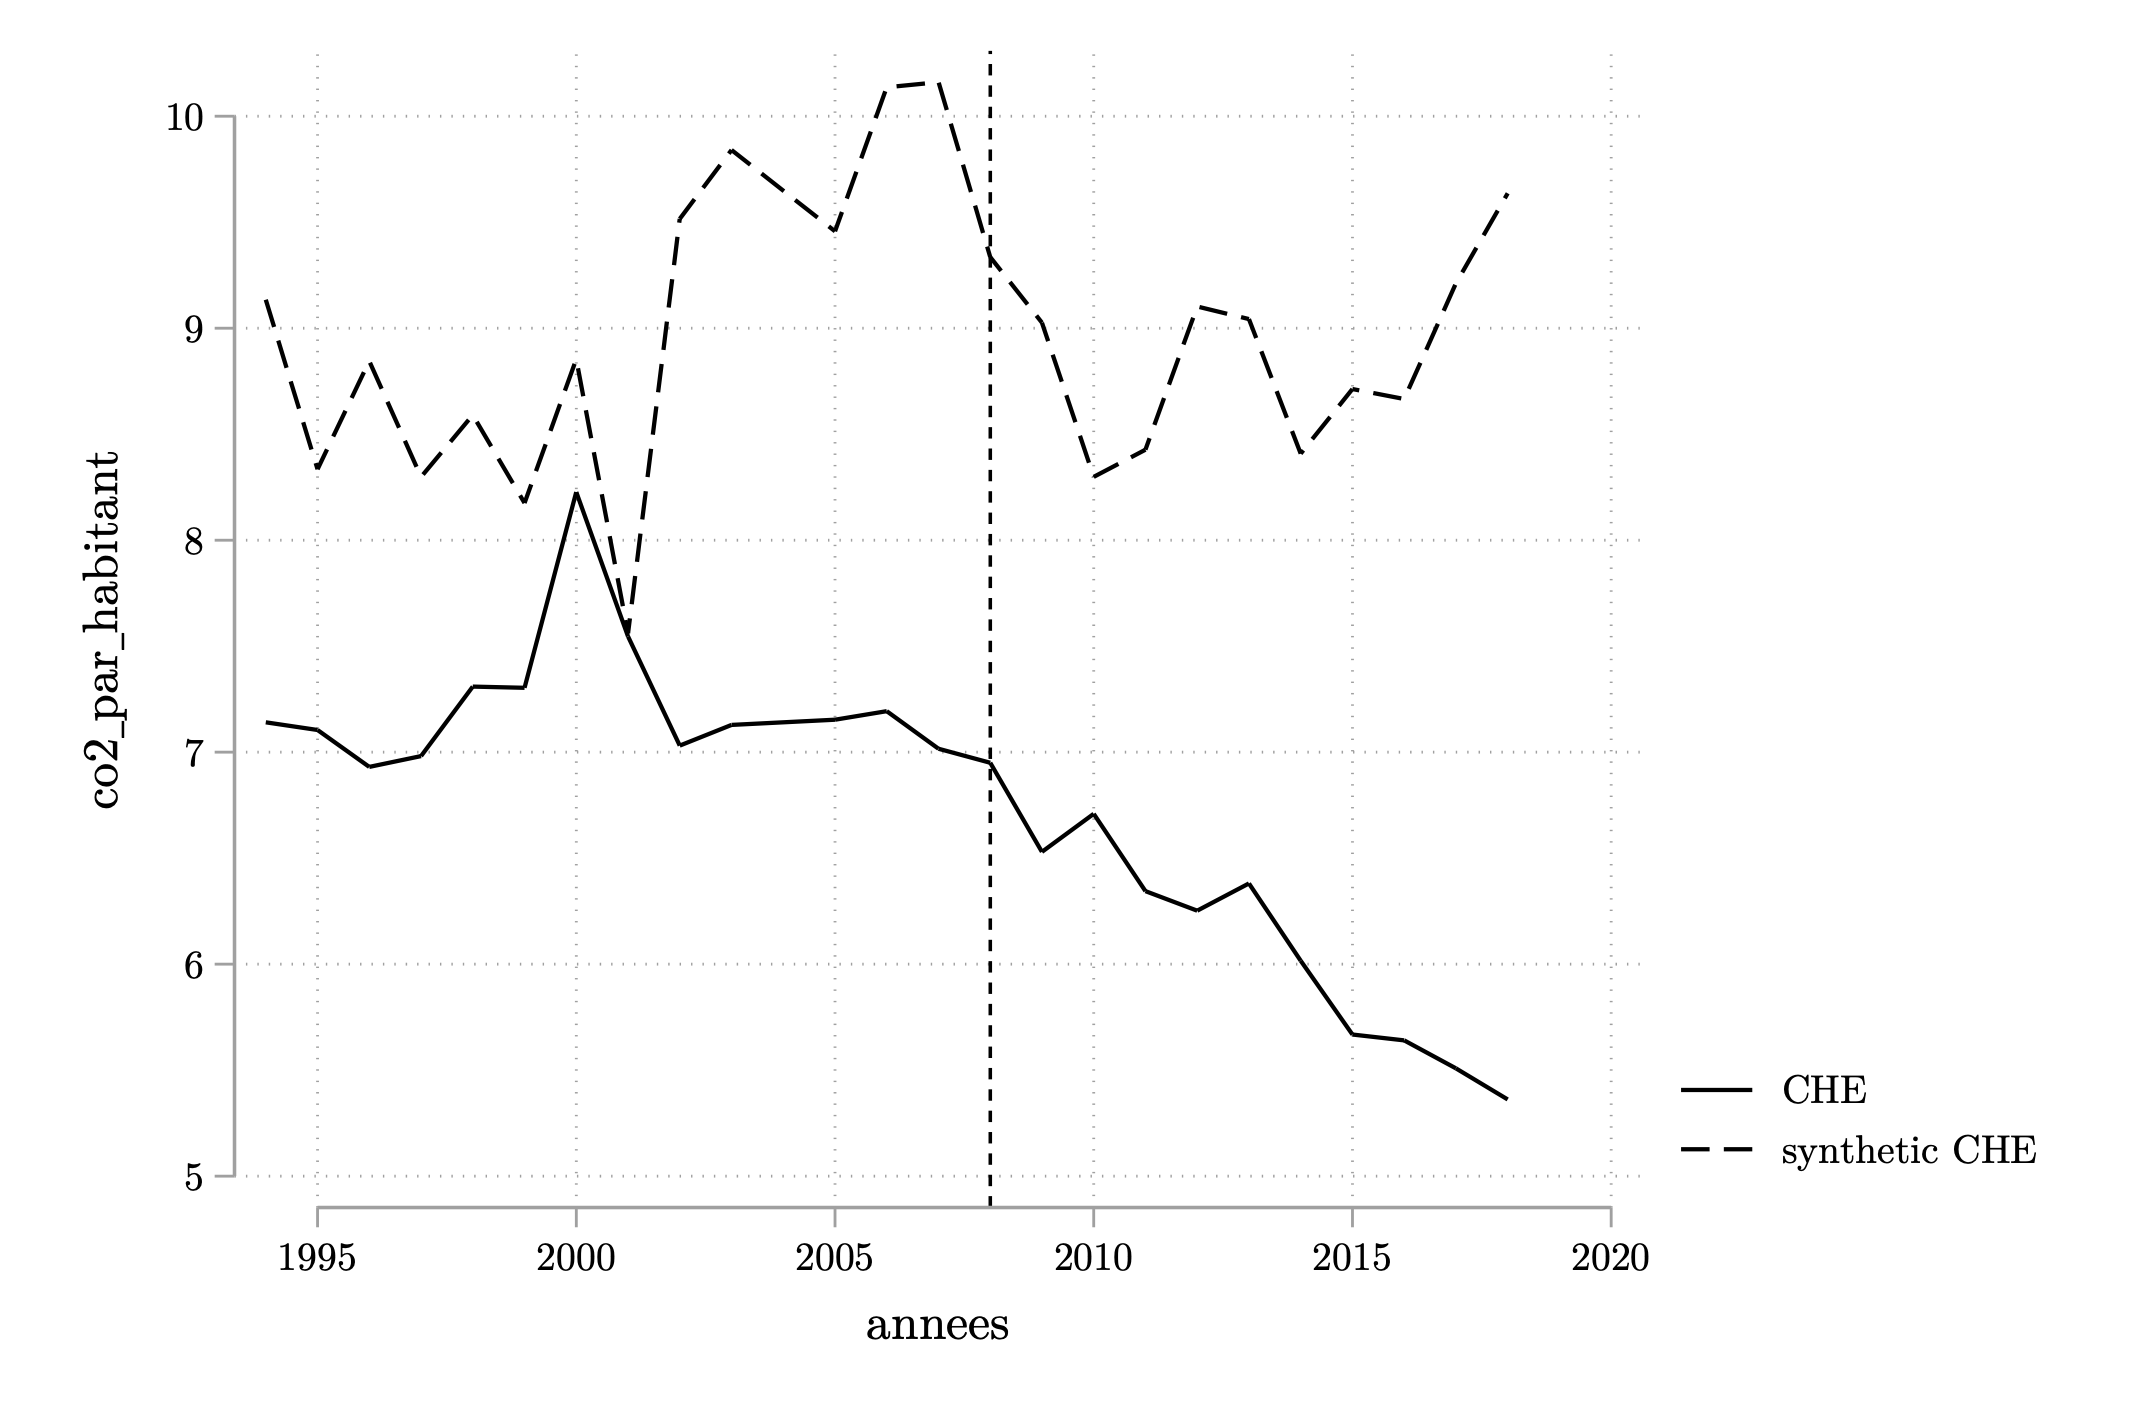
\includegraphics[width=0.6\textwidth]{Article/images/scm_omeans.png}
\caption{}
\label{fig:scm_omeans}
    \end{figure}


Les pondérations allouées dans la table \ref{tab:unit_weights} montrent que l'Autriche a la plus grande contribution (90.2\%), tandis que le Luxembourg n'a aucune contribution (0.0\%) et la Hollande une contribution minimale (9.8\%).

% Tableau des poids des unités
\begin{table}[ht]
\centering
\footnotesize{
\begin{tabular}{|l|*{2}{c}|}
\hline
            &  \_Co\_Number &   \_W\_Weight\\
\hline
AUT         &           1   &        .902\\
LUX         &           3   &           0\\
NLE         &           4   &        .098\\
\hline
\end{tabular}
}
\caption{}
\label{tab:unit_weights}
\end{table}

La table \ref{tab:RMSPE} montre un RMSPE de 1.981583 tonnes de CO2 par habitant, indiquant une erreur de prédiction considérable et suggérant que l'ajustement du modèle synthétique présente des écarts significatifs par rapport aux observations réelles.

% Tableau du RMSPE
\begin{table}[ht]
\centering
\footnotesize{
\begin{tabular}{|l|*{1}{c|}}
\hline
            &       RMSPE\\
\hline
RMSPE       &    1.981583\\
\hline
\end{tabular}
}
\caption{}
\label{tab:RMSPE}
\end{table}

Au vu des pondérations allouées (90.2 \% pour l'Autriche, 0.0 \% pour le Luxembourg, et 9.8 \% pour la Hollande) et d'un RMSPE\contentref{scm} de 1.981583$^{\left[\ref{tab:RMSPE}\right]}$  tonnes de CO2 par habitant, nous nous reposons sur le test initial des tendances parallèles qui a montré une violation de celles-ci. Bien que le résultat du SCM montre un effet négatif sur les émissions de CO2 (puisque le SCM est calculé comme la différence entre les émissions synthétiques et les émissions observées, \( y_{\text{synth, che}} - y_{\text{che}} \))\contentref{scm}, ce résultat suggère un impact négatif de la taxe CO2 très proche du résultat de la DiD. Cependant, en raison de la violation des tendances parallèles et des limitations méthodologiques associées, nous nous trouvons dans l'impossibilité de conclure à un effet causal robuste de la taxe CO2 sur les émissions de gaz à effet de serre en Suisse.


\subsection{Interprétation des résultats}

Les résultats indiquent une réduction significative des émissions de CO2 suite à l'introduction de la taxe CO2. Cependant, la violation des tendances parallèles dans l'analyse DiD et la forte dépendance à l'Autriche dans la SCM remettent en question la robustesse de ces conclusions. Bien que la taxe CO2 semble avoir un impact positif sur la réduction des émissions de gaz à effet de serre, les limitations méthodologiques observées suggèrent que ces résultats ne sont pas robustes. Il est donc crucial de continuer à affiner les méthodes d'évaluation pour obtenir des conclusions plus fiables.




%-------------------------------------------------------------------------%
% \newpage 
%-------------------------------------------------------------------------%